\section{RECOVERY}

\subsection{Airfield}

The standard VFR recovery for 108\th will be the overhead break, subject to
Tower permission. This is in theme with keeping "Navy".

\sidebyside{0.6}{%

  Altitude for the OHB is set by local airfield noise abatement process. With
  no other constraints it shall be 800 feet, in echelon, away from the tower,
  leader first, breaking away from the tower at midfield.  Note Kutaisi OHB
  altitude is 1500ft.

  Overhead breaks will break indicated by the Tower pattern (in airfield
  documentation) or away from populated areas or other runways, or to the left,
  and be done as a section in ten second intervals in the same manner as the
  Carrier break.

  For an IFR approaches refer to the published airfield documentation for a
  TACAN approach.

  When a whole flight lands in quick succession, the lead pilot will always
  take the hot lane which is the lane on the same side that the flight will
  leave the runway. Subsequent aircraft will stagger their landings on
  alternate sides of the runway.

}{%
  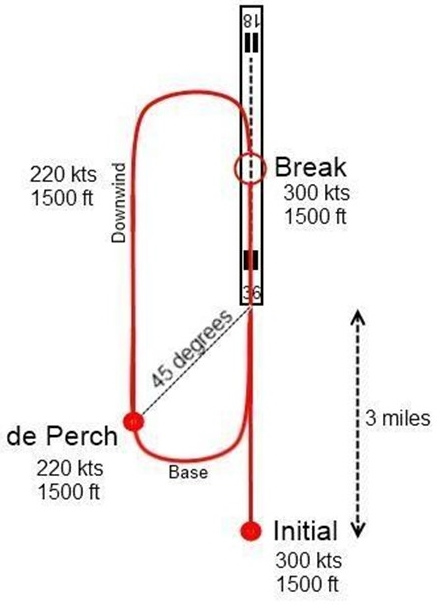
\includegraphics[width=\textwidth,align=t]{recovery/airfield}
}

Minimum spacing between sequentially landing aircraft is 3000 feet (0.5 nm), or
6000 feet (1 nm) with high wind or turbulence. Wake turbulence is currently
something to watch out for in tight sequences and the actual minimums could be
revised.

Formation approaches are not allowed if:

\begin{itemize}
  \item There is a crosswind component exceeding 15 kts
  \item The runway is wet or slippery
  \item The runway width is < 125 feet
  \item The weather has a ceiling lower than 500 feet AGL
  \item Asymmetric stores loadouts
  \item Unsafe loadouts like hung ordnance
\end{itemize}

It is also not recommended for night.

\subsection{Carrier}

See TTP-19 on the 132\nd website's documents page
